\documentclass[11pt, a4paper]{article}

\usepackage{amsmath}
\usepackage[a4paper, margin=1in]{geometry}
\usepackage{amsfonts}
\usepackage{mathtools}

\usepackage{tikz}
\usetikzlibrary{automata, positioning}

\usepackage{pgfplots}
\pgfplotsset{width=5cm,compat=1.9}

% remove paragraph indent
\setlength{\parindent}{0em}

% hyperlinks for the table of contents
% \usepackage{color}
% \usepackage{hyperref}
% \hypersetup{
    % colorlinks=true, % make the links colored
    % linkcolor=blue, % color TOC links in blue
    % urlcolor=red, % color URLs in red
    % linktoc=all % 'all' will create links for everything in the TOC
% }

\title{Probability Notes}

\begin{document}
    \maketitle{}
    \tableofcontents
    \newpage

    \pagenumbering{arabic}
    \section{Probability Theorems}
    \subsection{Set Theorems}
    For any three sets, the following hold true
    \begin{align*}
        A &= (A \cap B) \cup (A \cap B^{c}) \;where\;B\;and\;B^{c}\;are\;disjoint \\
        A \cap (B \cup C) &= (A \cap B) \cup (A \cap C) \\
        A \cup (B \cap C) &= (A \cup B) \cap (A \cup C)
    \end{align*}

    \subsection{Basic Probability Rules}
    \begin{align*}
        &\text{If } A \cap B = \phi \text{, then } P(A \cup B) = P(A) + P(B)\\
        &P(A|B)P(B) = P(B|A)P(A) = P(A \cap B) \tag*{Bayes' Theorem}\\
        &P(A) = P(A \cap B) + P(A \cap B^{c}) = P(A|B)P(B) + P(A|B^{c})P(B^{c})\\
        &P(A \cap B \cap C) = P(A) P(B|A) P(C|B,A) \tag*{Chain Rule}
    \end{align*}

    \subsubsection{Total Probability Theorem}
    Let $A_{1}$, $A_{2}$, .. ,$A_{n}$ be n disjoint events that completely cover the event space, and B be another event, then
    \begin{align*}
        P(B) &= P(B|A_{1})P(A_{1}) + P(B|A_{2})P(A_{2}) + \cdots + P(B|A_{n})P(A_{n})\\
        \text{or, } P(B) &= \sum_{i=1}^{n} P(B|A_{i})P(A_{i})
    \end{align*}
    \subsection{Independence}
    Two events A and B are independent iff
    \begin{align*}
        &P(A \cap B) = P(A) P(B)
    \end{align*}
    Note that \emph{independence} is not the same as \emph{disjoint}
    \begin{align*}
    A \cap B = \phi \Rightarrow P(A \cap B) = 0 \text{ but } P(A) \neq P(B) \neq 0
    \end{align*}
    Multiple events $A_{1}, A_{2}, \ldots , A_{n}$ are independent iff
    \begin{align*}
        P(A_{i} \cap A_{j} \cap \ldots \cap A_{k}) = P(A_{i}) P(A_{j}) \;..\; P(A_{k}) \;\;\forall\;i,j,\ldots,k \;|\; i,j,\ldots,k \in {1,2,\ldots,n}
    \end{align*}
    Conditional Independence is similar to the above equation. For an event C,
    \begin{align*}
        P(A_{i} \cap A_{j} \cap \ldots \cap A_{k} | C) = P(A_{i}|C) P(A_{j}|C) \;..\; P(A_{k}|C) \;\;\forall\;i,j,\ldots,k \;|\; i,j,\ldots,k \in {1,2,\ldots,n}
    \end{align*}
    
    \subsection{Joint Probability Distributions}
    \emph{Joint Probability Distributions} are defined for two or more than two variables. In this section, we only consider two variables. The formal definition is

    \begin{align*}
        P_{XY}(x, y) = P(X = x \;and\; Y = y)
    \end{align*}

    Based on this definition, the following theorems follow

    \begin{align*}
        \sum_{x} \sum_{y} P_{XY}(x,y) &= 1 \\
        P_{X}(x) &= \sum_{y} P_{XY}(x,y) \tag*{Marginal Probability} \\
        P_{X|Y}(x|y) &= P_{X|Y}(X=x|Y=y) = \frac{P_{XY}(x,y)}{P_{Y}{y}} \\
        \sum_{x} P_{X|Y}(x|y) &= 1 \tag*{Since Y is fixed and we sum over all X's} \\
        P_{XYZ}(x,y,z) &= P_{X}(x) P_{Y|X}(y|x) P_{Z|X,Y}(z|x,y) \tag*{Chain Rule}
    \end{align*}

    \subsection{Expected Value}
    Before going to expected value, let's define a Random Variable
    \begin{align*}
        \text{Random Variable } X \text{ is a linear map : } \mathbb{R} \to \mathbb{R} \text{. The value taken by the variable is denoted by } x
    \end{align*}
    
    $X$ will have an associated probability distribution, i.e., $P_{X}(X = x)$ . Using these quantities, we have
    \begin{align*}
        E[X] = \sum_x xP_{X}(X = x) \tag*{Expected Value}
    \end{align*}

    Based on this definition, the following theorems for expected value follow
    \begin{align*}
        E[\alpha] &= \alpha
        E[\alpha X] &= \alpha E[X] \\
        E[\alpha X + \beta] &= \alpha E[X] + \beta \\
        E[g(X)] &= \sum_x g(x)P_{X}(X = x) \\
        E[X^{2}] &= \sum_x x^{2} P_{X}(X = x) \tag*{Also called \emph{Second Moment}}\\
        E[X|A] &= \sum_{x} x P_{X|A}(X|A) \\
        E[g(X)|A] &= \sum_{x} g(x) P_{X|A}(X|A) \\
        E[X + Y + Z] &= E[X] + E[Y] + E[Z] \tag*{Linearity of Expectation}\\
        E[XY] &= \sum_{X} \sum_{Y} xy P_{XY}(x,y) \\
        E[g(X,Y)] &= \sum_{X} \sum_{Y} g(xy) P_{XY}(x,y) \\
        E[XY] &= E[X]E[Y] \tag*{if X and Y are \emph{independent}}
    \end{align*}
    where $\alpha, \beta \in \mathbb{R}$, $g(X) : \mathbb{R} \rightarrow \mathbb{R}$, and $A$ is an event, $X, Y, Z$ are Random Variables

    \subsubsection{Total Expectation Theorem}
    The \emph{Total Expectation Theorem} is the natural extension of the \emph{Total Probability Theorem}
    Let $A_{1}, A_{2}, \ldots, A_{n}$ be n disjoint events that completely cover the event space, and X be random variable, then
    \begin{align*}
        E[X] &= E[X|A_{1}]P(A_{1}) + E[X|A_{2}]P(A_{2}) + \cdots + E[X|A_{n}]P(A_{n})\\
        \text{or, } E[X)] &= \sum_{i=1}^{n} E[X|A_{i}]P(A_{i})
    \end{align*}

    \subsection{Variance}
    The formal definition of variance is
    \begin{align*}
        Var(X) = E[(X - \bar{X})^{2}] = E[X^{2}] - E[X]^{2}
    \end{align*}
    Using this definition, the following theorems follow
    \begin{align*}
        E[X^{2}] &= E[X]^{2} + Var(X) \\
        Var(\alpha) &= 0 \\
        Var(\alpha X + \beta) &= \alpha^{2} Var(X) \\
        Var(X + Y) &= Var(X) + Var(Y) \text{  if $X$ and $Y$ are \emph{independent} random variables}
    \end{align*}

    \subsection{Cumulative Probability Distribution}
    Cumulative probability distribution is defined for both discrete and continuous variables
    \begin{align*}
        F_{x}(X) = P(X \leq x) = \begin{cases} \int_{-\inf}^{x} p_{X}(t) dt &\mbox{$X$ is a discrete random variable}\\
                                               \sum_{k <= x} P_{X}(k) &\mbox{$X$ is a continuous random variable} \end{cases}
    \end{align*}



    \section{Binomial Random Variable}
    \emph{Binomial Random Variable} $X$ is defined as the number of successes in an experiment with $n$ independent trials, where each trial can only have two outcomes, \emph{success} or \emph{failure}.\\
    Let $X_{i}$ denote the Random Variable corresponding to the individual trials, with probability of success $p$. Then we have the following

    \begin{alignat*}{2}
        X_{i} &= \begin{cases} 1 &\mbox{if success in trial i}\\ 
                                0 &\mbox{otherwise} \end{cases} \tag*{indicator variable} \\
        X &= X_{1} + X_{2} + \cdots + X_{n} = \sum_{i=1}^{n} X_{i} \\
        P(X=k) &= \sum_{k=0}^{n} \binom{n}{k} p^{k} (1 - p)^{n-k}
    \end{alignat*}

    \subsection{Mean and Variance}
    First let's calculate the mean and variance for a single trial $X_{i}$
    \begin{alignat*}{2}
        E[X_{i}] &= 1 * p + 0 * (1 - p) &&= p\\
        Var(X_{i}) &= (1 - p)^{2}p + (0-p)^{2}(1-p) &&= p(1-p)
    \end{alignat*}
    
    We know that all $X_{i}'s$ are independent. Hence, the mean and variance for X become
    \begin{alignat*}{3}
        E[X] &= E[\sum_{i=1}^{n} X_{i}] &&= \sum_{i=1}^{n}E[X_{i}] &&= np \\
        Var(X) &= Var(\sum_{i=1}^{n} X_{i}) &&= \sum_{i=1}^{n} Var(X_{i}) &&= np(1-p)
    \end{alignat*}

    %%%%%%%%%%%%%%%%%%%%%%%%%%%%%%%%%%%%%%%%%%%%%%%%%%%%%%%%%%%%%%%%%%%%%%%%%%%
    \section{Continuous Uniform Random Variable}
    A uniform random variable is defined as follows
    \begin{align*}
        f_{X}(x) = \begin{cases} \frac{1}{b-a} &\mbox{$if a \leq x \leq b$}\\
                                    0 &\mbox{otherwise} \end{cases}
    \end{align*}

    \subsection{Mean and Variance}
    \begin{align*}
        E[X] &= \int_{a}^{b} x \frac{1}{b-a} dx = [\frac{x^{2}}{2(b-a)}]_{a}^{b}\\
            &= \frac{a+b}{2}\\
        Var(X) &= \int_{a}^{b} (x - \frac{a+b}{2})^{2} \frac{1}{b-a} dx \\
            &= \frac{(b-a)^{2}}{12}
    \end{align*}

    %%%%%%%%%%%%%%%%%%%%%%%%%%%%%%%%%%%%%%%%%%%%%%%%%%%%%%%%%%%%%%%%%%%%%%%%%%%
    \section{Gaussian Distribution}
    The gaussian distribution (or normal distribution) is defined between $-\inf$ and $\inf$. It is parametrized by mean $\mu$ and variance $\sigma$, $X \sim \mathcal{N}(\mu, \sigma^{2})$
    \begin{align*}
        f_{X}(x) = \frac{1}{\sqrt{2\pi \sigma^{2}}} e^{-\frac{(x-\mu)^{2}}{2 \sigma^{2}}}
    \end{align*}
    As already described,
    \begin{align*}
        E[X] &= \mu\\
        Var(X) &= \sigma^{2}
    \end{align*}

    A \emph{Standard Normal} is defined as a normal distribution with $\mu = 0$ and $\sigma^{2} = 1$\\
    Any normal distribution can be converted to a standard normal as $X = \frac{X - \mu}{\sigma}$\\
    If $Y = aX + b$, then $Y \sim \mathcal{N}(a \mu + b, a^{2}\sigma^{2})$

    %%%%%%%%%%%%%%%%%%%%%%%%%%%%%%%%%%%%%%%%%%%%%%%%%%%%%%%%%%%%%%%%%%%%%%%%%%%
    \section{Covariance and Correlation}
    For any two random variables X and Y,
    \begin{align*}
        Cov(X,Y) &= E[(X - \overline{X})(Y - \overline{Y})] = E[XY] - E[X]E[Y]\\
        Cov(X,X) &= Var(X)\\
        Corr(X,Y) &= E[(\frac{X - \overline{X}}{\sigma_{X}}) (\frac{Y - \overline{Y}}{\sigma_{Y}})]\\
        &= \frac{Cov(X,Y)}{\sigma_{X} \sigma_{Y}}
    \end{align*}
    Key points to note
    \begin{itemize}
        \item \emph{Inpdependence} $\Rightarrow Cov(X,Y) = Corr(X,Y) = 0$, but the converse is \emph{\textbf{not}} true
        \item Correlation is dimensionless and $-1 \leq Corr(X,Y) \leq 1$ with value close to $0$ implying minimal relation and values close to $-1, 1$ implying perfect relation
    \end{itemize}

    %%%%%%%%%%%%%%%%%%%%%%%%%%%%%%%%%%%%%%%%%%%%%%%%%%%%%%%%%%%%%%%%%%%%%%%%%%%
    \section{Iterated Expectation and Variance}
    The law of iterated expectation tells the following about expectation and variance
    \begin{align*}
        E[E[X|Y]] &= E[X] \\
        Var(X) &= E[Var(X|Y)] + Var(E[X|Y])\\
    \end{align*}

    Proof for Iterated Expectation
    \begin{align*}
        P(X) &= \sum_{y} P(X|Y) P(Y) \\
        \Rightarrow E[X] &= \sum_{x} xP(X) = \sum_{x} \sum{y} xP(X|Y)P(Y) \\
            &= \sum_{y} P(Y) \sum_{x} xP(X|Y) = \sum_{y} P(Y) E[X|Y] \\
        \text{or, } E[X] &= E[E[X|Y]] \tag*{$E[X|Y]$ is a function of $X$ and not $Y$}
    \end{align*}
    
    Proof for Variance
    \begin{align*}
        Var(X) &= E[X^{2}] - E[X]^{2} \\
        Var(X|Y) &= E[(X-\overline{X})^{2}|Y] = E[X^{2}|Y] - E[X|Y]^{2} \tag*{1}\\
        Var[E(X|Y)] &= E[E(X|Y)^{2}] - E[E[X|Y]]^{2}\\
                    &= E[E[(X|Y)]^{2}] - E[X]^{2} \tag*{2}\\
        E[Var(X|Y)] &= E[E[X^{2}|Y]] - E[E[X|Y]^{2}] \tag*{from 1}\\
                    &= E[X^{2}] - E[E[X|Y]^{2}] \tag*{3}\\
        E[Var(X|Y)] + Var(E[X|Y]) &= E[X^{2}] - E[X]^{2} \tag*{adding 2 and 3}\\
                                    &= Var(X)
    \end{align*}

    %%%%%%%%%%%%%%%%%%%%%%%%%%%%%%%%%%%%%%%%%%%%%%%%%%%%%%%%%%%%%%%%%%%%%%%%%%%
    \section{Random number of Random Variables}
    Let $X_{i}$ be independent identically distributed Random Variables and let $Y = \sum_{i=1}^{N} X_{i}$ be the sum of $N$ such random variables where $N$ itself is a random variable. Then,
    \begin{align*}
        Y &= X_{1} + X_{2} + \cdots + X_{N}\\
        E[Y|N=n] &= \sum_{i=1}^{n}E[X_{i}]\\
                &= NE[X]\\
        E[Y] &= E[E[Y|N]] = E[NE[X]]\\
            &= E[N]E[X] \tag*{since $E[X]$ will be a number}\\
        Var(Y) &= E[Var(Y|N)] + Var(E[Y|N])\\
            &= E[NVar(X)] + Var(NE[X])\\
            &= E[N]Var(X) + E[X]^{2}Var(N)
    \end{align*}

    %%%%%%%%%%%%%%%%%%%%%%%%%%%%%%%%%%%%%%%%%%%%%%%%%%%%%%%%%%%%%%%%%%%%%%%%%%%
    \section{Bernoulli Process}
    Bernoulli process falls under the family of random processes, which are random variables continuously evolving over time. Bernoulli process can be described as a sequence of independent Bernoulli trials, where each trial has only two outcomes : success with $P(success) = p$ and failure.
    \begin{alignat*}{2}
        P_{X_{t}}(x_{t}) &= \begin{cases} p &\mbox{if $X_{t} = 1$}\\
                                        1-p &\mbox{if $X_{t} = 0$} \end{cases}\\
        E[X_{t}] &= p\\
        Var(X_{t}) &= p(1-p)
    \end{alignat*}

    \subsection{Mean and Variance}
    Number of successes S in n time slots
    \begin{align*}
        P(S=k) &= \binom{n}{k} p^{k}(1-p)^(n-k)\\
        E[S] &= np\\
        Var(S) &= np(1-p)
    \end{align*}

    \subsection{Interarrival Times}
    Let $T_{1}$ denote the number of trials till the first success
    \begin{align*}
        P(T_{1} &= t) &= (1-p)^{t-1}p \tag*{$t \in {1, 2, \ldots}$}\\
        E[T_{1}] &= \frac{1}{p}\\
        Var(T_{1}) &= \frac{1-p}{p^{2}}
    \end{align*}
    This process is memoryless as all future coin flips are independent of whatever has happened till now. Also, the distribution is a \emph{Geometric Random Variable}.

    \subsection{Sum of Interarrival times}
    We are interested in the total time till k arrivals. Let this random variable be $Y_{k}$
    \begin{align*}
        Y_{k} &= T_{1} + T_{2} + \cdots + T_{k} \tag*{where $T_{i}$'s are i.i.d geometric with parameter $p$}\\
        P(Y_{k} = t) &= P(\text{$k-1$ arrivals between $t=1$ to $t=t$ and last arrival at time $t$})\\
           &= \binom{t-1}{k-1}p^{k}(1-p)^{t-k} \tag*{$\forall\; t \geq k$}\\
        E[Y_{k}] &= \sum_{i=1}{k}E[T_{i}]\\
                &= \frac{k}{p}\\
        Var(Y_{k}) &= \sum_{i=1}^{k}Var(T_{i})\\
                    &= \frac{k(1-p)}{p^{2}}
    \end{align*}


    %%%%%%%%%%%%%%%%%%%%%%%%%%%%%%%%%%%%%%%%%%%%%%%%%%%%%%%%%%%%%%%%%%%%%%%%%%%
    \section{Poisson Process}
    Poisson process also falls in the realm of random processes but is different from Bernoulli process as it is a continuous time process. This process is very commonly used to model arrival times and number of arrivals in a given time interval.
    \begin{align*}
        P(k, \tau) &= \text{Probability of $k$ arrivals in interval of duration $\tau$}\\
        \sum_{k} P(k, \tau) &= 1 \tag*{for a given $\tau$}
    \end{align*}
    Assumptions
    \begin{itemize}
        \item The Probability is dependent only on $\tau$ and not the \emph{location} of the interval
        \item Number of arrivals in disjoint time intervals are \emph{independent}
    \end{itemize}
    
    \subsection{Derivation from Bernoulli Process}
    For a very small interval $\delta$,
    \begin{alignat*}{2}
        P(k, \delta) &= \begin{cases} 1-\lambda \delta &\mbox{$k = 0$}\\
                                     \lambda \delta &\mbox{$k = 1$}\\
                                     0 &\mbox{$k > 2$} \end{cases} + O(\delta^{2})\\
        \lambda &= \lim_{\delta \to 0}\frac{P(1,\delta)}{\delta} \tag*{arrival rate per unit time}\\
        E[k] &= (\lambda \delta) * 1 + (1-\lambda \delta) * 0\\
            &= \lambda \delta \\
        \tau &= n \delta
    \end{alignat*}
    
    The last equation clearly implies that we can approximate the whole process as a bernoulli process where we have $n$ miniscule time intervals with at most one arrival per interval.
    \begin{align*}
        P(k\; arrivals) &= \binom{n}{k} p^{k} (1-p)^{n-k} \\
            &= \binom{n}{k} (\frac{\lambda \delta}{n})^{k} (1 - \frac{\lambda \delta}{n})^{n-k}\\
        \lambda \tau &= np \tag*{or, arrival rate * time = E[arrivals]}\\
        Poisson &= \lim_{\delta \to 0, n \to \inf} Bernoulli\\
        or,\; P(k, \tau) &= \frac{(\lambda \tau)^{k} e^{-\lambda \tau}}{k!} \tag*{$k = 0,1, \cdots$, for a given $\tau$}\\
        where,\; \sum_{k} P(k, \tau) &= 1 \tag*{for a given $\tau$}
    \end{align*}

    Let $N_{t}$ denote the no of arrivals till time t, then
    \begin{align*}
        E[N_{t}] &= \lambda t\\
        Var(N_{t}) &= \lambda t
    \end{align*}

    \subsection{Time till $k^{th}$ arrival}
    Suppose the $k^{th}$ arrival happens at a time $t$. Then we are saying that there have been $k-1$ arrivals till time $t$ and the $k^{th}$ arrival happens at time $t$ (precisely in an interval of $[t, t+\delta]$). Let $Y_{k}$ be the required time,
    \begin{align*}
        f_{Y_{k}}(t)\delta &= P(t \leq Y_{k} \leq t+\delta)\\
                    &= P(\text{$k-1$ arrivals  in $[0,t]$}) (\lambda \delta)\\
                    &= \frac{(\lambda t)^{k-1}}{(k-1)!}e^{-\lambda t}(\lambda \delta)\\
        f_{Y_{k}}(t) &= \frac{\lambda^{k} t^{k-1}}{(k-1)!}e^{-\lambda t} \tag*{Erland Distribution}
    \end{align*}

    \subsection{Time of $1^{st}$ arrival}
    Using the Erlang Distribution described above, we have
    \begin{align*}
        f_{Y_{1}}(t) = \lambda e^{-\lambda t}
    \end{align*}
    $Y_{k} = T_{1} + T_{2} + \cdots + T_{k}$ where all $T_{i}$ are independent and exponential distributions.

    \subsection{Merging of Poisson Processes}
    Merging of two Poisson processes is also a Poisson process. Consider two flasbulbs of Red and Green colours, flashing as Possion processes with rates $\lambda_{1}$ and $\lambda_{2}$. Then the process denoting the combined flashing of the two bulbs is also Poisson.\newline
    Consider a very small interval of time $\delta$. In this small interval, any of the individual bulbs can have at most one flashes (since we ignore higher order terms). Thus, the following four possibilities arise \newline
    \begin{table}[h]
    \centering
    \begin{tabular}{c|c|c}
        0 & $Red$ & $\overline{Red}$\\ \hline
        $Green$ & $\lambda_{1} \delta \lambda_{2} \delta $ & $(1-\lambda_{1}\delta)  \lambda_{2} \delta$\\ \hline
        $\overline{Green}$ & $\lambda_{1} \delta (1-\lambda_{2}\delta) $ & $(1-\lambda_{1}\delta) (1-\lambda_{2}\delta)$ \\
    \end{tabular}
    \caption{Base Probabilities for flashes}
    \end{table}
    \begin{table}[h]
    \centering
    \begin{tabular}{c|c|c}
        0 & $Red$ & $\overline{Red}$\\ \hline
        $Green$ & $0$ & $ \lambda_{2} \delta$\\ \hline
        $\overline{Green}$ & $\lambda_{1} \delta$ & $(1-(\lambda_{1} + \lambda_{2}) \delta)$ \\
    \end{tabular}
    \caption{Probabilities after ignoring $\delta^{2}$ terms}
    \end{table}

    Thus, the combined process is Poisson with parameter $\lambda_{1} + \lambda_{2}$ \newline
    \begin{align*}
    P(\text{arrival happened from first process}) = \frac{\lambda_{1} \delta}{\lambda_{1} \delta + \lambda_2 \delta} = \frac{\lambda_{1}}{\lambda_{1} + \lambda_{2}}
    \end{align*}

    \subsection{Splitting of Poisson Process}
    Suppose we have a Poisson process with parameter $\lambda$ which we split into two processes up and down, with probabilities $p$ and $1-p$. The two resulting processes are also Poisson with different parameters.\newline
    Consider a small time slot of length $\delta$. Then,
    \begin{align*}
        P(\text{arrival in this time slot}) &= \lambda \delta\\
        P(\text{arrival in up slot}) &= \lambda \delta p\\
        P(\text{arrival in down slot}) &= \lambda \delta (1-p)
    \end{align*}
    Thus, up and down are themselves Poisson with parameters $\lambda p$ and $\lambda (1-p)$ respectively.

    \subsection{Random Indcidence for Poisson}
    Suppose we have a Poisson process with parameter $\lambda$ running forever. We show up at a random time instant. What is the length of the chosen interarrival time (the total of the time from the last arrival to the next arrival).\newline
    Let $T_{1}^{'}$ denote the time that has elapsed since the last arrival and $T_{1}$ be the time till the next arrival. Note that the reverse process is also Poisson with the same parameter. Thus,
    \begin{align*}
        E[\text{interarrival time}] = E[T_{1}^{'} + T_{1}] = \frac{1}{\lambda} + \frac{1}{\lambda} = \frac{2}{\lambda}
    \end{align*}

    This may seem paradoxical since the time difference between any two arrivals in a Poisson process is same and it's expected length is $\frac{1}{\lambda}$, whereas we got an interval twice this length. The paradox is resolved by considering the fact that when we choose a random point in time, it is more likely to fall in an interval of larger size than the smaller ones (since probability will be proportional to the length of the interval).\newline

    Consider a separate example where we want to compare two values $E[\text{size of a family}]$ and $E[\text{size of a family of a given person}]$.\newline
    The two value will be different due to the underlying nature of the way experiment is conducted. For the first, we randomly choose families and average their sizes. Here, family of any size is equally likely to be picked. In the second case, we first pick a person from the population, get their family size, and then average the sizes of the families. Note that, this experiment is biased since the we are more likely to select people from larger families (or equivalently, it is more likely that we pick a person from a large family since the probability of picking is proportional to the family size). Hence, the second value will likely be larger and the two quantities are not equal.


    %%%%%%%%%%%%%%%%%%%%%%%%%%%%%%%%%%%%%%%%%%%%%%%%%%%%%%%%%%%%%%%%%%%%%%%%%%%
    \section{Markov Process}
    Markov Process is a discrete time process that is not memoryless. Here the random variable takes several possible states, and the probability distribution is defined in such a way that $P(\text{transition from state 1 to state 2})$ is dependent on state 1.\newline

    Let $X_{n}$ be the random variable denoting the state after n transitions and $X_{0}$ will represent the starting state (which can be given or random). Markov assumption states that \emph{Given the current state, past does not matter}. Armed with these,
    \begin{align*}
        p_{ij} &= P(\text{next state $j$ $|$ current state $i$})\\
        p_{ij} &= P(X_{n+1}=j|X_{n}=i) = P(X_{n+1}=j|X_{n}=i, X_{n-1}, \ldots, X_{0})\\
        r_{ij}(n) &= P(X_{n}=j|X_{0}=i) \tag*{or, in state $j$ after $n$ steps}\\
        r_{ij}(n) &= \sum_{k=1}^{m} r_{ik}(n-1)p_{kj}
    \end{align*}

    \subsection{Recurring and Transient States}
    A state $i$ is called \emph{recurrent} if, starting from $i$, and travelling anywhere, it is always possible to return to $i$. If a state is not recurrent, it is \emph{transient}. States in a recurrent class are periodic if they can be grouped into $d > 1$ groups so that all transitions from one group lead to the next group.

    \subsection{Steady State Probabilities}
    Do $r_{ij}(n)$ converge to some $\pi_{j}$ (independent of i) ? \newline
    Yes if,
    \begin{itemize}
        \item recurrent states are all in a single class
        \item single recurrent class is not periodic (otherwise oscillations are possible)
    \end{itemize}
    Assuming yes,
    \begin{align*}
        r_{ij}(n) &= \sum_{k} r_{ik}(n-1)p_{kj}\\
        \lim_{n \to \inf} r_{ij}(n) &= \sum_{k} r_{ik}(n-1)p_{kj}\\
        \pi_{ij} &= \sum_{k} \pi_{ik} p_{kj} \tag*{balance equations} \\
        \sum_{i} \pi_{i} &= 1 \\
        \text{frequency of transitions $k \rightarrow j$} &= \pi_{k} p_{kj} \tag*{in one step}\\
        \text{frequency of transitions into $j$} &= \sum_{k} \pi_{k} p_{kj} \tag*{influx from all connected states}e
    \end{align*}

    \subsection{Birth Death Process}
    Consider the checkout counter example. The states are represented by the number of people currently being processed, and we always move $n$ to $[n-1, n, n+1]$, i.e., either the people in the queue decrease by one, remain same or increase by one. Let the probability for moving up be $p$ and moving down be $q$.

    \begin{center}
    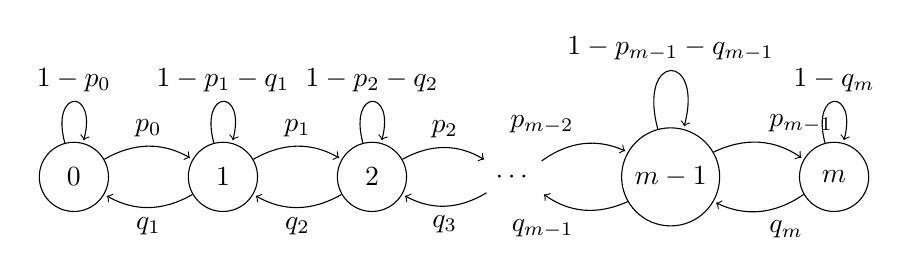
\begin{tikzpicture}
        % first add the node that we want to represent
        \node[state]             (0) {$0$};
        \node[state, right=of 0] (1) {$1$};
        \node[state, right=of 1] (2) {$2$};
        \node[draw=none, right=of 2] (3) {$\cdots$};
        \node[state, right=of 3] (4) {$m-1$};
        \node[state, right=of 4] (5) {$m$};
        % draw the edges between the nodes
        % bend left/right is from the persepective of the starting node
        % and so is the auto=left/right which specifies the side to put text
        \draw[every loop]
            % right edges
            (0) edge[bend left, auto=left] node {$p_{0}$} (1)
            (1) edge[bend left, auto=left] node {$p_{1}$} (2)
            (2) edge[bend left, auto=left] node {$p_{2}$} (3)
            (3) edge[bend left, auto=left] node {$p_{m-2}$} (4)
            (4) edge[bend left, auto=left] node {$p_{m-1}$} (5)
            % left edges
            (1) edge[bend left, auto=left] node {$q_{1}$} (0)
            (2) edge[bend left, auto=left] node {$q_{2}$} (1)
            (3) edge[bend left, auto=left] node {$q_{3}$} (2)
            (4) edge[bend left, auto=left] node {$q_{m-1}$} (3)
            (5) edge[bend left, auto=left] node {$q_{m}$} (4)
            % self loops
            (0) edge[loop above] node {$1-p_{0}$} (0)
            (1) edge[loop above] node {$1-p_{1}-q_{1}$} (1)
            (2) edge[loop above] node {$1-p_{2}-q_{2}$} (2)
            (4) edge[loop above] node {$1-p_{m-1}-q_{m-1}$} (4)
            (5) edge[loop above] node {$1-q_{m}$} (5);
    \end{tikzpicture}
    \end{center}

    Let's estimate the steady state probabilities. Consider the following diagram splitting the chain into two parts through the two adjacent states
    \begin{center}
    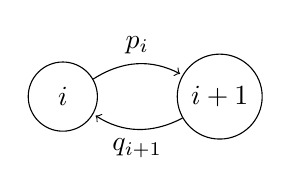
\begin{tikzpicture}
        % first add the node that we want to represent
        \node[state]             (0) {$i$};
        \node[state, right=of 0] (1) {$i+1$};
        % draw the edges between the nodes
        % bend left/right is from the persepective of the starting node
        % and so is the auto=left/right which specifies the side to put text
        \draw[every loop]
            % right edges
            (0) edge[bend left, auto=left] node {$p_{i}$} (1)
            % left edges
            (1) edge[bend left, auto=left] node {$q_{i+1}$} (0);
    \end{tikzpicture}
    \end{center}

    In this case, to maintain steady state, long term frequency of left-right transition should be same as right left transition, i.e., $\pi_{i}p_{i} = \pi_{i+1}q_{i}$ \newline
    In the special case of $p_{i} = p$ and $q_{i} = q \;\forall\; i$,
    \begin{align*}
        \rho &= \frac{p}{q} \tag*{load factor}\\
        \pi_{i+1} &= \pi_{i} \frac{p}{q} = \pi_{i} \rho \\
        \pi_{i} &= \pi_{0} \rho^{i} \tag*{$i = 0,\ldots,m$} \\
        \text{Using } \sum_{i=0}^{m} \pi_{0}\rho^{i} &= 1,\\
        \pi_{0} &= \frac{1}{\sum_{i=0}^{m} \rho^{i}}\\
        \text{if $p < q$ and $m \rightarrow \inf,$}\\
        \pi_{0} &= 1 - \rho \\
        \pi_{i} &= (1-\rho)\rho^{i}\\
        E[X_{n}] &= \frac{\rho}{1-\rho} \tag*{Exponential Distribution}
    \end{align*}
    When $\rho = 1$ or $p = q$, then all states are equally likely - symmetric random walk.

    \subsection{Absorption Probabilities}
    let $a_{i}$ denote the probability of absorption and $\mu_{i}$ denote the expected no of steps until absorption starting from state $i$. Then,
    \begin{align*}
        a_{i} &= \sum_{j} a_{j}p_{ij} \tag*{outflux to the possible states}\\
        \mu_{i} &= 1 + \sum_{j} \mu_{j} p_{ij}
    \end{align*}
    For multipe absorption states, we can possibly consider them together as a group and calculate the relevant quantities. \newline
    For a given state $s$,
    \begin{align*}
        E[\text{steps to first time reach $s$ from $i$}] &= t_{i} \\
        t_{i} &= E[min \{n \geq 0 \text{ such that } X_{n} = s\}] \\
        t_{s} &= 0 \\
        t_{i} &= 1 + \sum_{j} t_{j}p_{ij} \tag*{outflux to all possible states}
    \end{align*}

    Mean recurrence time (mean time to reach back a state) for $s$
    \begin{align*}
        t_{s}^{*} &= E[min\{n \geq 1 \text{ such that } X_{n}=s\} | X_{0} = s] \\
        t_{s}^{*} &= 1 + \sum_{j} t_{j} p_{ij}
    \end{align*}

    %%%%%%%%%%%%%%%%%%%%%%%%%%%%%%%%%%%%%%%%%%%%%%%%%%%%%%%%%%%%%%%%%%%%%%%%%%%
    \subsection{Weak Law of Large Numbers}
    Suppose we want to know the mean height of penguins in the world. The absolutely correct answer can be obtained by taking the average of the entire population. But ths is not practical, and often we will have to resort to estimating the quantity through a sample. Let there be $n$ penguins in the sample and $X_{1}, X_{2}, \ldots, X_{n}$ be the random variables denoting their heights. Then,
    \begin{align*}
        M_{n} &= \frac{X_{1} + X_{2} + \cdots + X_{n}}{n}\\
        \lim_{n \to \inf} E[M_{n}] &= E[X] = \text{The true mean}
    \end{align*}

    \subsection{Markov Inequality/Chebychev Inequality}
    For nonnegative random variable $X$,
    \begin{alignat*}{2}
        E[X] &= \sum_{x}xp_{X}(x) &&\geq \sum_{x \geq a}xp_{X}(x) \tag*{discrete case}\\
            &= \int_{x}xp_{X}(x) &&\geq \int_{x \geq a}xp_{X}(x) \tag*{continuous case}
    \end{alignat*}
    
    Applying the above set of inequalities to the variable $X - \mu$
    \begin{align*}
        E[(X - \mu)^{2}] &\geq a^{2} P((X - \mu)^{2} \geq a^{2}) \\
        \text{or, \;} Var(X) &\geq a^{2} P(\mid X - \mu \mid \geq a)\\
        \text{For continuous case, }\\
        \sigma^{2} &= \int_{-\inf}^{\inf} (x-\mu)^{2}f_{X}(x) dx\\
                  &\geq \int_{-\inf}^{\mu-c} (x-\mu)^{2}f_{X}(x)dx + \int_{\mu+c}^{\inf} (x-\mu)^{2}f_{X}(x)dx\\
                  &\geq c^{2} P(\mid X - \mu \mid \geq c)\\
        \text{Hence,}\\
        P(\mid X - \mu \mid \geq c^{2}) &\leq \frac{\sigma^{2}}{c^{2}}\\
        \text{or, } \\
        \Aboxed{P(\mid X - \mu \mid \geq k\sigma) &\leq \frac{1}{k^{2}}}\text{\;\;\;where $c = k\sigma$}
    \end{align*}

    Going back to the problem of estimating the mean,
    \begin{align*}
        M_{n} &= \frac{X_{1} + X_{2} + \cdots + X_{n}}{n} \\
        E[M_{n}] &= \frac{1}{n} \sum_{i=1}^{n} E[X_{i}] = \mu \text{\;\; expectation of expectation} \\
        Var(M_{n}) &= \sum_{i=1}^{n} Var(\frac{X_{i}}{n}) = \frac{\sigma^{2}}{n} \text{\;\; since $X_{i}$ are independent} \\
        \Aboxed{P(\mid M_{n} - \mu \mid \geq \epsilon) &\leq \frac{\sigma^{2}}{n\epsilon^{2}}}
    \end{align*}
    or, as $n \rightarrow \inf,\; M_{n} - \mu \rightarrow 0$, $\epsilon$ is the error bound/confidence.

    %%%%%%%%%%%%%%%%%%%%%%%%%%%%%%%%%%%%%%%%%%%%%%%%%%%%%%%%%%%%%%%%%%%%%%%%%%%
    \section{Central Limit Theorem}
    Chebychev's inequality gives a loose bound. We can do better with CLT. Let $X$ be a random variable with mean $\mu$ and variance $\sigma^{2}$, and let $X_{i}$ be independent identically distributed random variables with the same distribution as $X$. Then,
    \begin{align*}
        S_{n} &= X_{1} + X_{2} + \cdots + X_{n}\\
        Z_{n} &= \frac{S_{n} - E[S_{n}]}{\sigma_{n}} \text{\;\;random variable with mean $0$ and variance $1$} \\
             &= \frac{S_{n} - nE[X]}{\sqrt{n} \sigma}\\
        \text{or,\;\;} S_{n} &= \sqrt{n} \sigma Z_{n} + nE[X] \\
        \text{In\;\;} \lim_{n \to \inf} Z_{n} &\rightarrow Z \text{\;(standard normal)}\\
        \text{or,\;\;} \Aboxed{Z &= \frac{S_{n} - nE[X]}{\sqrt{n} \sigma}} \text{\;\;only for CDF (no comment on PDF/PMF)}\\
        \text{Thus,\;\;} \Aboxed{P(Z > c) &= P(\frac{S_{n} - nE[X]}{\sqrt{n} \sigma} > c)}
    \end{align*}
    By defining the confidence on how close we desire $S_{n}$ to the actual mean, we can calculate the required value of the $n$ using standard normal CDF tables. However, we need to have an estimate of variance of the distribution in order to do the estimate of $n$.


    %%%%%%%%%%%%%%%%%%%%%%%%%%%%%%%%%%%%%%%%%%%%%%%%%%%%%%%%%%%%%%%%%%%%%%%%%%%
    \section{Bayesian Inference}
    We have a signal $S$ that goes through a "model" $a$ through which we observe $X$ (with sum added noise $N$). The aim of Bayesian Inference is to try to infer $S$ given the observed $X$.
    \newline
    Hypothesis testing is done on an unknown that takes some possible values, and the aim is to arrive at a value that gives a small probability of incorrect decision (e.g. - Radar)
    \newline
    Estimation is aimed at finding the value of a quantity with a small estimation error (e.g. poll estimation)
    \newline
    Bayes Rule
    \begin{align*}
        p_{\Theta|X}(\theta|x) &= \frac{p_{\Theta}(\theta)p_{X|\Theta}(x|\theta)}{p_{X}(x)} \tag*{$\theta$ and $X$ are both discrete}\\
        \text{or,\;\;} Posterior &= \frac{Prior * Model}{Data}\\
        p_{\Theta|X}(\theta|x) &= \frac{p_{\Theta}(\theta)f_{X|\Theta}(x|\theta)}{f_{X}(x)} \tag*{$\theta$ is discrete and $X$ is continuous}\\
    \end{align*}
    Note that Bayesian inference will give us a distribution over the possible values, but it is often desirable to get an estimate.

    \subsection{Maximum a Posteriori (MAP)}
    MAP is a point estimate of the unknown quantity and is defined as follows
    \begin{align*}
        p_{\Theta|X}(\theta|x) = \max_{\theta}p_{\Theta|X}(\theta|x) \tag*{$\theta$ with maximum posterior probability}\\
    \end{align*}
    In continuous case, expected value can be a better estimate

    \subsection{Least Mean Square Estimate}
    Here, we aim to find an estimate such that
    \begin{align*}
        \theta* &= \min_{c} E[(\Theta - c)^{2}]\\
        E[(\Theta - c)^{2}] &= E[\Theta^{2}] - 2cE[\Theta] + c^{2}\\
        \text{Taking derivative,\;\;} \frac{dE}{dc} &= 0\\
        \Aboxed{c &= E[\Theta]}\\
        \text{In general,\;\;} c &= E[\Theta|X] \tag*{minimizes $E[(\Theta - g(X))^{2}]$ over all estimators $g(X)$ }
    \end{align*}
    $E[\Theta]$ minimizes the least squares estimate
    \newline
    When $X$ is observed, the best estimate simlply becomes $E[\Theta|X]$.


    %%%%%%%%%%%%%%%%%%%%%%%%%%%%%%%%%%%%%%%%%%%%%%%%%%%%%%%%%%%%%%%%%%%%%%%%%%%
    \section{Problems}
    \subsection{Cumulative Distribution Function}
    A random variable X is a combination of a continuous and discrete distribution as follows
    \begin{align*}
        f_{X}(x) = \begin{cases} 0.5 &\mbox{$a \leq x \leq b$}\\
                                 0.5 &\mbox{x = 0.5}\\
                                 0 &\mbox{otherwise} \end{cases}
    \end{align*}
    Find the Cumulative Distribution of X.\newline \newline
    
    \textbf{Ans.} Cumulative Distribution of X can be found by integration and is as follows
    \begin{align*}
        f_{X}(x) = \begin{cases} 0 &\mbox{$x < 0$}\\
                                 0.5x &\mbox{$0 \leq x < 0.5$}\\
                                 0.75 &\mbox{x = 0.5}\\
                                 0.75 + 0.5(x-0.5) &\mbox{$0.5 < x \leq 1$} \\
                                 1 &\mbox {$1 < x$}\end{cases}
    \end{align*}

    %%%%%%%%%%%%%%%%%%%%%%%%%%%%%%%%%%%
    \subsection{Number of tosses till first head}
    When tossing a fair coin, what is the $E[\#\;tosses\;till\;the\;first\;H]$ ?\newline \newline
    \textbf{Ans.} Let $X$ be the \# of tosses till first \emph{H}. Then, $(X = 1) \cap (X > 1) = \phi$.\\
    Using \emph{Total Expectation Theorem}
    \begin{align*}
        E[X] &= P(X = 1)E[X|X = 1] + P(X > 1)E[X|X > 1] \\
        &= 0.5 * 1 + 0.5 E[X] \\
        \Rightarrow E[X] &= 2
    \end{align*}
    $P(X = 1) = 0.5$ because then we get the head in the first toss itself. Since $P(X = 1) + P(X > 1) = 1$, we have $P(X > 1) = 0.5$. $E[X] = E[X|X > 1]$ because the tosses are \emph{independent} and thus memoryless.
    
    %%%%%%%%%%%%%%%%%%%%%%%%%%%%%%%%%%%
    \subsection{Iterated Expectation practice}
    A class has two sections denoted by the random variable $Y$. Let $X$ denote the quiz score of a student. Given that section 1 has 10 students, section 2 has 20 students, $E[X|Y=1] = 90 E[X|Y=2] = 60, Var(X|Y=1) = 10, Var(X|Y=2) = 20$, find $E[X]$ and $Var(X)$.\newline \newline
    \textbf{Ans.} We use the formulae from iterated expectation to calculate these.
    \begin{alignat*}{2}
        P_{Y}(y) &= \begin{cases} \frac{1}{3} &y = 1\\
                                \frac{2}{3} &y = 2 \end{cases}\\
        E[X] &= E[E[X|Y]] = \sum_{y}E[X|Y]P(Y)\\
            &= 90 * \frac{1}{3} + 60 * \frac{2}{3}\\
        Var(X) &= E[Var(X|Y)] + Var(E[X|Y])\\
              &= \sum_{y}Var(X|Y)P(Y) + ((90-E[E[X|Y])^{2}\frac{1}{3} + (60-E[E[X|Y]])^{2}\frac{2}{3})\\
              &= \frac{650}{3}
    \end{alignat*}

    %%%%%%%%%%%%%%%%%%%%%%%%%%%%%%%%%%%
    \subsection{Hat Problem}
    $n$ people throw their hats in a box and then pick a hat at random. What is the expected number of people who pick their own hat ?\newline \newline
    \textbf{Ans.} Let $X$ denote the number of people who pick their own hat. We have been asked $E[X]$.\\
    Let $X_{i}$ be a binary random variable denoting whether the $i^{th}$ person picked their own hat, i.e.,
    \begin{alignat*}{2}
        X_{i} &= \begin{cases} 1 &\mbox{if $i^{th}$ person picks their own hat}\\ 
                                0 &\mbox{otherwise} \end{cases} \\
        P(X_{i} = 1) &= \frac{1}{n} \\
        E[X_{i}] &= 1 * \frac{1}{n} + 0 * (1 - \frac{1}{n}) = \frac{1}{n}\\
    \end{alignat*}
    Consequently
    \begin{align*}
        E[X] = E[\sum_{i=1}^{n} X_{i}] = \sum_{n=1}^{n}E[X_{i}] = 1
    \end{align*}

    It is interesting to see the variance of X. Note that the formula for variance is $E[X^{2}] - E[X]^{2}$. Thus,
    \begin{align*}
        X^{2} = (\sum_{i=1}^{n} X_{i})^{2} = \sum_{i=1}^{n} X_{i}^{2} + \sum_{i=1}^{n} \sum_{j=1, j\neq i}^{n} X_{i}X{_j} \\
        E[X^{2}] = \sum_{i=1}^{n}E[X_{i}^{2}] + \sum_{i=1}^{n} \sum_{j=1, j\neq i}^{n} E[X_{i}X{_j}] 
    \end{align*}
    Note that $X_{i}$ and $X_{j}$ are not independent since after the first person has picked the hat, only $n-1$ hats remain
    \begin{alignat*}{3}
        X_{i}X_{j} &= \begin{cases} 1 &\mbox{if $X_{i} = X_{j} = 1$}\\
                                   0 &\mbox{otherwise} \end{cases} \\
        P(X_{i}X_{j} = 1) &= P(X_{i} = 1) P(X_{j} = 1|X_{i} = 1) &&= \frac{1}{n} * \frac{1}{n-1}\\
        E[X_{i}X_{j}] &= 1 * (\frac{1}{n} * \frac{1}{n-1}) + 0 * (1 - \frac{1}{n} * \frac{1}{n-1}) &&= \frac{1}{n(n-1)}\\
        E[X_{i}^2] &= 1^{2} \frac{1}{n} + 0^{2} (1-\frac{1}{n}) &&= \frac{1}{n}
    \end{alignat*}
    Putting these values in the original equation for variance
    \begin{alignat*}{2}
        E[X_{2}] &= n \frac{1}{n} + \frac{1}{n} \frac{1}{n-1} (\frac{n(n-1)}{2} * 2) &&= 2\\
        Var(X) &= 2 - 1^{2} &&= 1
    \end{alignat*}

    %%%%%%%%%%%%%%%%%%%%%%%%%%%%%%%%%%%
    \subsection{Breaking a stick}
    A stick of length $l$ is broken first at $X$ uniformly chosen between $[0,l]$, and then at $Y$, uniformly chosen between $[0,X]$. Find the expected length of the shorter part.\newline \newline
    \textbf{Ans.} The following is the joint probability distribution of $X$ and $Y$
    \begin{align*}
        f_{XY}(x, y) = f_{X}(x) f_{Y|X}(y|x) = \frac{1}{l} \frac{1}{x} = \frac{1}{xl} \;\forall\; 0 \leq y \leq x \leq 1
    \end{align*}
    
    Using marginal probabilities, we can calculate $f_{Y}(y) and E[Y] as$
    \begin{align*}
        f_{Y}(y) = \int f_{XY}(x,y) dx = \int_{y}^{l} \frac{1}{xl} dx = \frac{1}{l} \log \frac{l}{y} \tag*{Note that for any $y$, $y \leq x \leq l$}\\
        E[Y] = \int y f_{Y}(y) = \int_{0}{l} y \frac{1}{l} \log\frac{l}{y} = \frac{l}{4}
    \end{align*}

    This problem can also be approched using iterated expectation
    \begin{align*}
        E[Y] &= E[E[Y|X]] = E[\text{uniform random variable between $0$ and $x$}]\\
            &= E[\frac{X}{2}] =\frac{1}{2}E[X]\\
            &= \frac{l}{4} 
    \end{align*}

    %%%%%%%%%%%%%%%%%%%%%%%%%%%%%%%%%%%
    \subsection{PMF of g(X)}
    Let $X$ be uniform in $[0, 2]$, then find the PMF of $Y = X^{3}$. \newline \newline
    \textbf{Ans.} Always solve such questions using the cumulative distribution approach.
    \begin{alignat*}{2}
        P(X \leq x) &= \begin{cases} 0 &\mbox{$x < 0$}\\
                                    \frac{1}{2} x &\mbox{$0 \leq x \leq 2$}\\
                                    1 &\mbox{$2 < x$} \end{cases}\\
        P(Y \leq y) &= P(X^{3} \leq y) = P(X \leq y^{\frac{1}{3}})\\
                    &= \begin{cases}  0 &\mbox{$y < 0$}\\
                                        \frac{1}{2} y^{\frac{1}{3}} &\mbox{$0 \leq y^{\frac{1}{3}} \leq 2$}\\
                                        1 &\mbox{$2 < y^{\frac{1}{3}}$} \end{cases}\\
        f_{Y}(y) &= \frac{dP(Y <= y)}{dy}(y)\\
                 &= \begin{cases}  0 &\mbox{$y < 0$}\\
                                        \frac{1}{6} y^{\frac{-2}{3}} &\mbox{$0 \leq y \leq 8$}\\
                                        0 &\mbox{$8 < y$} \end{cases}
    \end{alignat*}

    %%%%%%%%%%%%%%%%%%%%%%%%%%%%%%%%%%%
    \subsection{Poisson Emails}
    You get emails according to a Poisson process at the rate of 5 messages/hour. You check email every 30 minutes. Find \newline
    \begin{itemize}
        \item P(no new message)
        \item P(one new message)
    \end{itemize}
    \textbf{Ans.} We can model the arrival process like a Poisson process. $\lambda = 5$ and $\tau = \frac{1}{2}$\\
    \begin{align*}
            P(\lambda, \tau, k) &= \frac{(\lambda \tau)^{k} e^{-\lambda \tau}}{k!} \\
            P(5, \frac{1}{2}, 0) &= \frac{(5 * \frac{1}{2})^{0} e^{-5 * \frac{1}{2}}}{0!} \\
            P(5, \frac{1}{2}, 1) &= \frac{(5 * \frac{1}{2})^{1} e^{-5 * \frac{1}{2}}}{1!}
    \end{align*}

    %%%%%%%%%%%%%%%%%%%%%%%%%%%%%%%%%%%
    \subsection{Poisson Fishing}
    We go fishing where we catch fishes at the rate of $0.6/hour$. We fish for two hours. If we do not catch a fish in the first two hours, we fist until the first catch. Find the following
    \begin{itemize}
        \item P(fish for $> 2$ hours)
        \item P(fish for $> 2$ but $< 5$ hours)
        \item P(catch at least two fish)
        \item E[fish]
        \item E[Total fishing time]
        \item E[future fishing time|fished for two hours]
    \end{itemize}
    \textbf{Ans.}
    \begin{itemize}
        \item P(fish for $> 2$ hours) = $P(k=0, \tau=2)$ = $e^{-0.6 * 2}$
        \item P(fish for $> 2$ but $< 5$ hours) = P(first catch in $[2,5]$ hours) = $P(k=0,\tau=2)(1-P(k=0,\tau=3)$ which is no fish in $[0,2]$ but at least $1$ fish in the next $3$ hours (which will be independent of first $2$ hours)
        \item P(catch at least two fish) = P(at least $2$ catches before $2$ hours) = $1 - P(k=0,\tau=2) - P(k=1,\tau=2)$
        \item E[fish] has two possibilities, either single fish after $2$ hours, or many fist before $2$ hours. $E[fish] = E[fish|\tau \leq 2](1-P(\tau > 2)) + E[fish|\tau > 2] P(\tau > 2) = (0.6*2)*(1-P(k=0,\tau=2)) + 1*P(k=0,\tau=2)$
        \item E[Total fishing time] = $2 + P(k=0,\tau=2)\frac{1}{\lambda}$, since we fish for atlest $2$ hours
        \item E[future fishing time|fished for two hours] can be obtained using the memoryless property of Poisson process. The expected time till first arrival is independent of what has happened till now. Thus, $E[T_{1}] = \frac{1}{\lambda}$
    \end{itemize}


    %%%%%%%%%%%%%%%%%%%%%%%%%%%%%%%%%%%
    \subsection{Poisson Lightbulbs}
    We have three identical but independent lightbulbs whose lifetimes are modelled by a Poisson process with parameter $\lambda$. Given that we start all the three bulbs together, find the $E[\text{time until last bulb dies out}]$ \newline \newline
    \textbf{Ans.} Start with the merged Poisson process which will denote the time till the first bulb will fail. For this process, $\lambda^{'} = 3\lambda$. Hence, $E[\text{first bulb fails}] = \frac{1}{3\lambda}$.\newline
    After the first bulb dies out, we are left with a process with $\lambda^{'} = 3\lambda$. Due to memoryless property, $E[\text{second bulb fails}] = \frac{1}{2\lambda}$ and consequently $E[\text{last bulb fails}] = \frac{1}{\lambda}$. \newline
    Note the above two times denote the time difference, i.e. the time taken for the bulb to die out after the last bulb died out. Thus, $E[\text{time until last bulb dies out}] = \frac{1}{3\lambda} + \frac{1}{2\lambda} + \frac{1}{\lambda}$

    
    %%%%%%%%%%%%%%%%%%%%%%%%%%%%%%%%%%%
    \subsection{Steady State Markov Process}
    Find the steady state probabilites of the following Markov Process\newline
    \begin{center}
    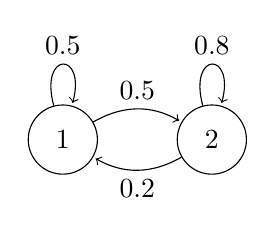
\begin{tikzpicture}
        % first add the node that we want to represent
        \node[state]             (1) {$1$};
        \node[state, right=of 1] (2) {$2$};
        % draw the edges between the nodes
        % bend left/right is from the persepective of the starting node
        % and so is the auto=left/right which specifies the side to put text
        \draw[every loop]
            % right edges
            (1) edge[bend left, auto=left] node {$0.5$} (2)
            % left edges
            (2) edge[bend left, auto=left] node {$0.2$} (1)
            % self loops
            (1) edge[loop above] node {$0.5$} (1)
            (2) edge[loop above] node {$0.8$} (2);
    \end{tikzpicture}
    \end{center}
    
    \textbf{Ans.} Using balance equations, we have
    \begin{align*}
        \pi_{1} &= \pi_{1}p_{11} + \pi_{2}p_{21}\\
        \pi_{2} &= \pi_{1}p_{12} + \pi_{2}p_{22}\\
        \pi_{1} + \pi_{2} &= 1
    \end{align*}
    Solving, $\pi_{1} = \frac{2}{7}$ and $\pi_{2} = \frac{5}{7}$
    
    %%%%%%%%%%%%%%%%%%%%%%%%%%%%%%%%%%%
    \subsection{Absorption Probabilities}
    \begin{center}
    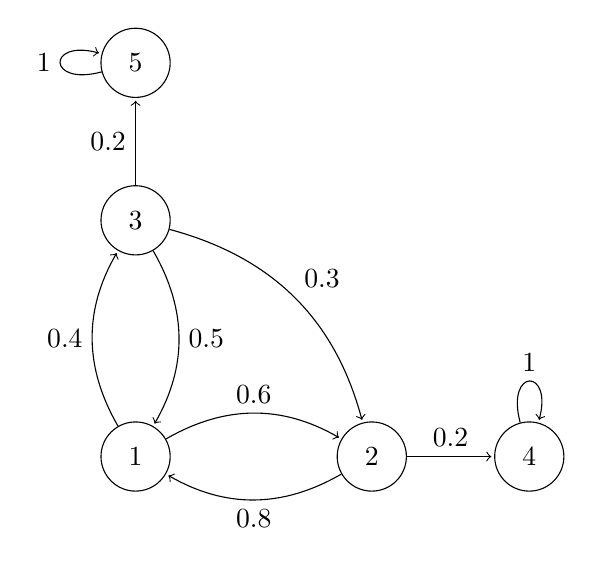
\begin{tikzpicture}
        % first add the node that we want to represent
        \node[state] at (0,0)     (5) {$5$};
        \node[state] at (0,-2)    (3) {$3$};
        \node[state] at (0,-5)    (1) {$1$};
        \node[state] at (3,-5)    (2) {$2$};
        \node[state] at (5,-5)    (4) {$4$};
        % draw the edges between the nodes
        % bend left/right is from the persepective of the starting node
        % and so is the auto=left/right which specifies the side to put text
        \draw[every loop]
            % 5
            (5) edge[loop left] node {$1$} (5)
            % 3
            (3) edge[auto=left]            node {$0.2$} (5)
            (3) edge[bend left, auto=left] node {$0.5$} (1)
            (3) edge[bend left, auto=left] node {$0.3$} (2)
            % 1
            (1) edge[bend left, auto=left] node {$0.4$} (3)
            (1) edge[bend left, auto=left] node {$0.6$} (2)
            % 2
            (2) edge[bend left, auto=left] node {$0.8$} (1)
            (2) edge[auto=left]            node {$0.2$} (4)
            %4
            (4) edge[loop above] node {$1$} (4);
    \end{tikzpicture}
    \end{center}    
    Calculate the absorption probabilites for state $4$ and expected time to absortion from all states. (for absorption time, assume $p_{35} = 0$ and $p_{32} = 0.5$\newline \newline
    \textbf{Ans.} Let $a_{i}$ denote the abosorption probabilites into state $4$ starting from $i$
    \begin{align*}
        a_{5} &= 0, a{4} = 1 \\
        a_{i} &= \sum_{j} a_{j}p_{ij}\\
        a_{2} &= a_{1}p_{21} + a_{4}p_{24}\\
        a_{3} &= a_{1}p_{31} + a_{2}p_{32} + a_{5}p_{35}\\
        a_{1} &= a_{2}p_{12} + a_{3}p_{13}
    \end{align*}
    Solving, $a_{1} = \frac{9}{14}, a_{2} = \frac{5}{7}$ and $a_{3} = \frac{15}{28}$ \newline
    
    Let $\mu_{i}$ denote the expected time till absorption starting from $i$, then
    \begin{align*}
        \mu_{4} &= 0 \\
        \mu_{1} &= 1 + \mu_{2}p_{12} + \mu_{3}p_{13} \\
        \mu_{2} &= 1 + \mu_{1}p_{21} + \mu_{4}p_{24} \\
        \mu_{3} &= 1 + \mu_{1}p_{31} + \mu_{2}p_{32}
    \end{align*}
    Solving, $\mu_{1} = \frac{55}{4}, \mu_{2} = 12$ and $\mu_{3} = \frac{111}{8}$ \newline

    
    %%%%%%%%%%%%%%%%%%%%%%%%%%%%%%%%%%%
    \subsection{Estimating Binomial with CLT, $\frac{1}{2}$ correction}
    Given a Bernoulli Process with $n = 36$ and $p = 0.5$, find $P(S_{n} <= 21)$. \newline \newline
    \textbf{Ans.} The exact answer will be
    \begin{align*}
        \sum_{k=0}^{21}\binom{36}{k}(\frac{1}{2})^{36} = 0.8785
    \end{align*}
    But the same can be estimated using the CLT as follows
    \begin{align*}
        \mu = np = 18\\
        \sigma^{2} = np(1-p) = 9\\
        P(S_{n} \leq 21) \approx P(\frac{S_{n} - 18}{3} \leq \frac{21-18}{3}) \approx 0.843
    \end{align*}
    Our estimate is in the rough range of the answer but not quite close. We can do better using the $\frac{1}{2}$ correction
    \begin{align*}
        P(S_{n} \leq 21) = P(S_{n} < 22) \text{\;\;since $S_{n}$ is an integer}\\
        \text{Consider \;}P(S_{n} <= 21.5) \text{\;\;as a compromise between the two}\\
        P(S_{n} <= 21.5) = P(\frac{S_{n} - 18}{3} \leq \frac{21.5 - 18}{3}) \approx 0.879
    \end{align*}
    In a similar manner, $P(S_{n}=19) = P(18.5 \leq S_{n} \leq 19.5)$ using $\frac{1}{2}$ correction.


    %%%%%%%%%%%%%%%%%%%%%%%%%%%%%%%%%%%
    \subsection{LMS estimate}
    Given the prior $f_{\Theta|(\theta)}$, uniform in $[4,10]$, and $f_{X|]Theta}(x|\theta)$ is uniform in $[\theta-1, \theta+1]$, estimate the posterior of $\theta$.
    \newline \newline
    \textbf{Ans.} we need to evaluate $f_{\Theta|X}(\theta|x)$ in order to get $E[\Theta|X]$.
    \newline
    $f_{X,\Theta}(x,\theta) = f_{X}(x) f_{\Theta|X}(\theta|x)$ which is a parallelogram on the $\theta-x$ plane at the points  $(3,4)$, $(5,4)$, $(9,10)$ and $(11,10)$. Then $E[\Theta|X]$ can be obtained by drawing vertical lines on the planes and calculating the $E[\theta]$ over that line. It is a line which bends at two points.

    % plot of f(theta)
    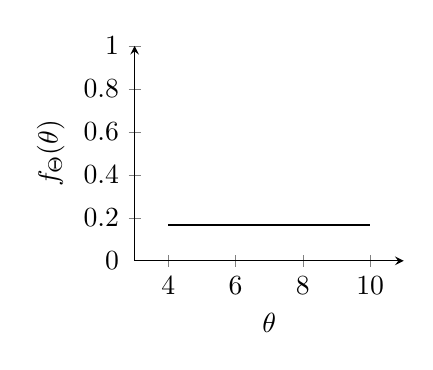
\begin{tikzpicture}
        \begin{axis}[
            axis lines = left,
            xlabel = $\theta$,
            ylabel = {$f_{\Theta}(\theta)$},
            xmin=3, xmax=11,
            ymin=0, ymax=1
        ]
        %define the plot here
        \addplot [
            domain=4:10, 
            samples=2, 
            color=black,
        ]
        {1/6};
        \end{axis}
    \end{tikzpicture}
    \hskip 5pt
    % plot of f(X|theta)
    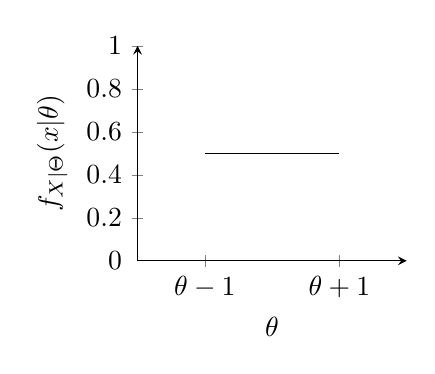
\begin{tikzpicture}
        \begin{axis}[
            axis lines = left,
            xlabel = $\theta$,
            ylabel = {$f_{X|\Theta}(x|\theta)$},
            xmin=0, xmax=4,
            ymin=0, ymax=1,
            xticklabels={$\theta-1$,$\theta+1$},
            xtick={1,3}
        ]
        %define the plot here
        \addplot [
            domain=1:3,
            samples=2, 
            color=black,
        ]
        {1/2};
        \end{axis}
    \end{tikzpicture}
    \hskip 5pt
    % plot of theta vs x
    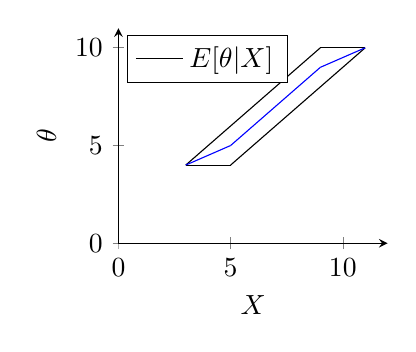
\begin{tikzpicture}
        \begin{axis}[
            axis lines = left,
            xlabel = $X$,
            ylabel = {$\theta$},
            xmin=0, xmax=12,
            ymin=0, ymax=11,
            legend pos=north west,
        ]
        %define the plot here
        \addplot [
            domain=3:5,
            samples=2, 
            color=black,
        ]
        {4};
        \addplot [
            domain=3:9,
            samples=2, 
            color=black,
        ]
        {x+1};
        \addplot [
            domain=9:11,
            samples=2, 
            color=black,
        ]
        {10};
        \addplot [
            domain=5:11,
            samples=2, 
            color=black,
        ]
        {x-1};
        % \addlegendentry{$\theta\;vs\;x$}
        \addplot [
            domain=3:5,
            samples=2, 
            color=blue,
        ]
        {(x/2)+(5/2)};
        \addplot [
            domain=5:9,
            samples=2, 
            color=blue,
        ]
        {x};
        \addplot [
            domain=9:11,
            samples=2, 
            color=blue,
        ]
        {(x/2)+(9/2)};
        \addlegendentry{$E[\theta|X]$}
        \end{axis}
    \end{tikzpicture}


    %%%%%%%%%%%%%%%%%%%%%%%%%%%%%%%%%%%
    %%%%%%%%%%%%%%%%%%%%%%%%%%%%%%%%%%%

\end{document}